\documentclass[conference]{IEEEtran}
\IEEEoverridecommandlockouts
% \usepackage{cite} % Already present
\usepackage{amsmath,amssymb,amsfonts}
\usepackage{algorithmic}
\usepackage{graphicx}
\usepackage{textcomp}
\usepackage{xcolor}
\usepackage{float} % Added for H placement option
% It's good practice to ensure inputenc and fontenc are set for potential non-ASCII characters in names/text
\usepackage[utf8]{inputenc}
\usepackage[T1]{fontenc}

\def\BibTeX{{\rm B\kern-.05em{\sc i\kern-.025em b}\kern-.08em
    T\kern-.1667em\lower.7ex\hbox{E}\kern-.125emX}}

\begin{document}

\title{Implementasi Metode Newton-Raphson untuk Menentukan Kecepatan Optimal Drone Guna Memaksimalkan Jangkauan dalam Bahasa C++}

\author{
    \IEEEauthorblockN{Andi M. Alvin F.}
    \IEEEauthorblockA{\textit{NPM: 2306161933} \\
    \textit{Universitas Indonesia}\\
    Depok, Indonesia}
\and
    \IEEEauthorblockN{Daffa Sayra Firdaus}
    \IEEEauthorblockA{\textit{NPM: 2306267151} \\
    \textit{Universitas Indonesia}\\
    Depok, Indonesia}
\and
    \IEEEauthorblockN{Fathan Yazid Satriani}
    \IEEEauthorblockA{\textit{NPM: 2306250560} \\
    \textit{Universitas Indonesia}\\
    Depok, Indonesia}
\and
    \IEEEauthorblockN{Rowen Rodotua Harahap}
    \IEEEauthorblockA{\textit{NPM: 2306250604} \\
    \textit{Universitas Indonesia}\\
    Depok, Indonesia}
\and
    \IEEEauthorblockN{Ryan Adidaru Excel B.}
    \IEEEauthorblockA{\textit{NPM: 2306266994} \\
    \textit{Universitas Indonesia}\\
    Depok, Indonesia}
}

\maketitle

\begin{abstract}
Laporan ini membahas implementasi metode Newton-Raphson untuk menyelesaikan persamaan non-linear $f(v)=0$ yang berkaitan dengan optimasi parameter penerbangan drone. Fokus utama adalah pada penentuan kecepatan terbang optimal ($v$) untuk memaksimalkan jangkauan. Studi kasus menggunakan model daya drone dimana $P(v) = c_1v^3 + c_2/v$ (menggunakan $c_1, c_2$ untuk konsistensi dengan implementasi), dan untuk jangkauan maksimum dicari akar dari $f(v) = \frac{d(P(v)/v)}{dv} = 2c_1v - 2c_2v^{-3} = 0$. Implementasi dilakukan dalam bahasa C++ dengan analisis konvergensi dan perbandingan terhadap solusi analitik $v = (c_2/c_1)^{1/4}$. Data input untuk pengujian dihasilkan secara sintetis dan dibaca dari file eksternal.
\end{abstract}

\begin{IEEEkeywords}
metode Newton-Raphson, optimasi drone, kecepatan optimal, pemrograman numerik, C++
\end{IEEEkeywords}

\section{Pendahuluan}
Optimasi dalam operasi drone memainkan peran krusial dalam meningkatkan efisiensi dan efektivitas misi penerbangan. Salah satu aspek penting adalah penentuan kecepatan terbang optimal untuk memaksimalkan jangkauan operasional. Masalah ini dapat diformulasikan sebagai pencarian akar dari persamaan non-linear yang merepresentasikan kondisi optimal.

Metode numerik, khususnya metode Newton-Raphson, menawarkan pendekatan yang efektif untuk menyelesaikan persamaan non-linear tersebut. Metode ini dipilih karena konvergensinya yang cepat (kuadratik) ketika tebakan awal cukup dekat dengan solusi.

Tujuan dari proyek ini adalah mengimplementasikan metode Newton-Raphson dalam bahasa C++ untuk menemukan kecepatan optimal drone, mengujinya dengan berbagai set parameter drone yang dihasilkan secara sintetis, dan menganalisis hasil serta konvergensinya.

\section{Studi Literatur}
\subsection{Metode Newton-Raphson}
Metode Newton-Raphson adalah teknik iteratif untuk mencari akar fungsi real $f(x)$ menggunakan formula:
\begin{equation}
x_{i+1} = x_i - \frac{f(x_i)}{f'(x_i)}
\end{equation}
Dalam konteks optimasi kecepatan drone, variabel $x$ diganti dengan $v$ sehingga:
\begin{equation}
v_{i+1} = v_i - \frac{f(v_i)}{f'(v_i)}
\end{equation}
Interpretasi geometris dari metode ini adalah menemukan titik potong antara garis singgung pada suatu titik dengan sumbu-x, yang secara iteratif akan menuju ke akar fungsi.

\subsection{Kriteria Konvergensi}
Iterasi dihentikan ketika salah satu kriteria berikut terpenuhi:
\begin{itemize}
\item Perubahan absolut antara iterasi berturut-turut, $|v_{i+1} - v_i|$, kurang dari toleransi yang ditentukan ($\epsilon$).
\item Jumlah iterasi mencapai batas maksimum yang ditetapkan.
\end{itemize}
Kriteria lain seperti $|f(v_i)| < \text{toleransi}$ juga dapat digunakan, namun implementasi ini berfokus pada perubahan $v$.

\subsection{Model Daya Drone}
Model daya drone yang digunakan adalah:
\begin{equation}
P(v) = c_1v^3 + \frac{c_2}{v}
\end{equation}
dimana:
\begin{itemize}
\item $c_1$: koefisien terkait gaya hambat parasitik.
\item $c_2$: koefisien terkait gaya hambat terinduksi.
\item $v$: kecepatan terbang.
\end{itemize}

\section{Data Yang Digunakan}
\subsection{Fungsi Target}
Untuk memaksimalkan jangkauan, kita mencari kecepatan $v$ dimana turunan dari rasio daya per kecepatan ($P(v)/v$) terhadap $v$ sama dengan nol:
\begin{equation}
f(v) = \frac{d(P(v)/v)}{dv} = 2c_1v - 2c_2v^{-3} = 0
\end{equation}
Turunan pertama $f(v)$ terhadap $v$ adalah $f'(v)$, yang dibutuhkan untuk metode Newton-Raphson:
\begin{equation}
f'(v) = 2c_1 + 6c_2v^{-4}
\end{equation}

\subsection{Parameter Input dan Generasi Data}
Parameter input untuk setiap kasus uji meliputi:
\begin{itemize}
    \item Koefisien $c_1$ dan $c_2$: berdasarkan karakteristik fisik drone.
    \item Tebakan awal $v_0$: nilai positif yang masuk akal untuk kecepatan drone.
    \item Toleransi error $\epsilon$: misalnya $10^{-5}$.
    \item Jumlah iterasi maksimum: misalnya 100.
\end{itemize}
Data input ini ($c_1, c_2, v_0, \epsilon, \text{max\_iter}$) disimpan dalam file teks bernama \texttt{synthetic\_data.txt}. Setiap baris dalam file ini merepresentasikan satu set parameter uji. File ini dihasilkan oleh program C++ terpisah (\texttt{data.cpp} yang dikompilasi menjadi \texttt{generate\_data}), yang membuat sejumlah set data sesuai input pengguna. Program \texttt{generate\_data} menghasilkan nilai $c_1, c_2,$ dan $v_0$ secara acak dalam rentang yang ditentukan, sementara $\epsilon$ diatur ke $10^{-5}$ dan iterasi maksimum ke 100.

Format per baris dalam \texttt{synthetic\_data.txt}: \texttt{c1 c2 v0\_awal epsilon iterasi\_maks}.

\section{Metode Yang Digunakan}
\subsection{Algoritma Newton-Raphson}
\begin{algorithmic}[1]
\STATE Input: $c_1, c_2, v_0, \epsilon, \text{max\_iter}$
\STATE $v_{\text{current}} \gets v_0$
\STATE $i \gets 0$
\WHILE{$i < \text{max\_iter}$}
    \STATE Hitung $f_{\text{val}} = f(v_{\text{current}}, c_1, c_2)$
    \STATE Hitung $df_{\text{val}} = f'(v_{\text{current}}, c_1, c_2)$
    \IF{$|df_{\text{val}}| < \text{nilai\_sangat\_kecil}$}
        \STATE Return error "Derivative Zero"
    \ENDIF
    \STATE $v_{\text{next}} \gets v_{\text{current}} - f_{\text{val}} / df_{\text{val}}$
    \IF{$v_{\text{next}} \le 0$}
        \STATE Return error "Non-Positive Velocity"
    \ENDIF
    \IF{$|v_{\text{next}} - v_{\text{current}}| < \epsilon$}
        \STATE Return $v_{\text{next}}$ (Konvergen)
    \ENDIF
    \STATE $v_{\text{current}} \gets v_{\text{next}}$
    \STATE $i \gets i + 1$
\ENDWHILE
\STATE Return $v_{\text{current}}$ (Max Iterations Reached)
\end{algorithmic}
Algoritma ini juga mencakup pemeriksaan untuk kondisi input yang tidak valid ($v_0 \le 0$, $c_1 \le 0$, atau $c_2 \le 0$) sebelum iterasi dimulai.

\section{Diskusi dan Analisa Hasil Experimen}

\subsection{Implementasi Kode Program}
Kode program C++ utama (\texttt{main.cpp}) yang digunakan untuk analisis komprehensif adalah sebagai berikut. Program ini membaca data parameter dari file \texttt{synthetic\_data.txt} yang dihasilkan sebelumnya.
\begingroup % Start a group to keep the font size change local
\tiny % Or \footnotesize, \scriptsize, \tiny
\begin{verbatim}
#include <iostream>
#include <cmath>
#include <iomanip>
#include <vector>
#include <string>
#include <fstream> // Required for file input
#include <sstream> // Required for parsing lines from file

// Function to calculate f(v) = 2*c1*v - 2*c2*v^(-3)
// This function represents the derivative of (Power/Velocity) 
// with respect to v, set to 0 for optimal range.
double f_drone(double v, double c1, double c2) {
    if (v <= 1e-9) { 
        return 1e12; 
    }
    return 2.0 * c1 * v - (2.0 * c2 / (v * v * v));
}

// Function to calculate f'(v) = 2*c1 + 6*c2*v^(-4)
// This is the derivative of f_drone(v) with respect to v.
double df_drone(double v, double c1, double c2) {
    if (v <= 1e-9) {
        return 1e12; 
    }
    return 2.0 * c1 + (6.0 * c2 / (v * v * v * v));
}

// Structure to hold results for each test case
struct TestCaseResult {
    double c1_param; 
    double c2_param; 
    double v0_initial;
    double v_optimal_numerical;
    int iterations_taken;
    double v_optimal_analytical;
    double relative_error_percent;
    std::string status_message;
};

// Newton-Raphson implementation for finding optimal drone speed
TestCaseResult newton_raphson_solver(double c1, double c2, 
                                     double v0, double tolerance, 
                                     int max_iter, 
                                     bool print_iterations_detail = false) {
    double v_current = v0;
    int iter = 0;
    TestCaseResult result = {c1, c2, v0, v0, 0, 0.0, -1.0, 
                             "Max Iterations Reached"};

    if (v0 <= 0) {
        result.status_message = "Invalid Initial Guess (v0 <= 0)";
        return result;
    }
     if (c1 <= 0 || c2 <= 0) {
        result.status_message = "Invalid Parameters (c1 or c2 <= 0)";
        return result;
    }    if (print_iterations_detail) {
        std::cout << "\n--- Iteration Details for c1=" << c1 
                  << ", c2=" << c2 << ", v0=" << v0 << " ---\n";
        std::cout << std::setw(10) << "Iteration"
                  << std::setw(18) << "v_i (m/s)"
                  << std::setw(18) << "f(v_i)"
                  << std::setw(18) << "f'(v_i)"
                  << std::setw(18) << "v_{i+1} (m/s)"
                  << std::setw(20) << "|v_{i+1}-v_i|" << std::endl;
        std::cout << std::string(102, '-') << std::endl;
    }

    while (iter < max_iter) {
        double f_val = f_drone(v_current, c1, c2);
        double df_val = df_drone(v_current, c1, c2);

        if (std::abs(df_val) < 1e-10) { 
            if (print_iterations_detail) 
                std::cerr << "Error: Derivative too close to zero at v = " 
                          << v_current << std::endl;
            result.status_message = "Derivative Zero";
            result.v_optimal_numerical = v_current;
            result.iterations_taken = iter;
            return result;
        }

        double v_next = v_current - f_val / df_val;
        double change = std::abs(v_next - v_current);

        if (v_next <= 0) { 
             if (print_iterations_detail) 
                std::cerr << "Error: Next velocity is non-positive (v_next = " 
                          << v_next << ")" << std::endl;
            result.status_message = "Non-Positive Velocity";
            result.v_optimal_numerical = v_current; 
            result.iterations_taken = iter;
            return result;
        }

        if (print_iterations_detail) {
            std::cout << std::fixed << std::setprecision(8)
                      << std::setw(10) << iter
                      << std::setw(18) << v_current
                      << std::setw(18) << f_val
                      << std::setw(18) << df_val
                      << std::setw(18) << v_next
                      << std::setw(20) << change << std::endl;
        }

        if (change < tolerance) {
            if (print_iterations_detail) 
                std::cout << "\nConverged after " << iter + 1 
                          << " iterations!" << std::endl;
            result.status_message = "Converged";
            result.v_optimal_numerical = v_next;
            result.iterations_taken = iter + 1;
            return result;
        }

        v_current = v_next;
        iter++;
    }

    if (print_iterations_detail) 
        std::cerr << "Warning: Maximum iterations (" << max_iter 
                  << ") reached without convergence." << std::endl;
    result.v_optimal_numerical = v_current; 
    result.iterations_taken = iter;
    return result;
}

void print_summary_table(const std::vector<TestCaseResult>& results) {
    std::cout << "\n\n--- Summary Table of Newton-Raphson Results" << std::endl;
    std::cout << std::setw(10) << "c1"
              << std::setw(10) << "c2"
              << std::setw(15) << "v0_initial"
              << std::setw(20) << "v_optimal_num"
              << std::setw(12) << "Iterations"
              << std::setw(20) << "v_optimal_analyt"
              << std::setw(18) << "Rel.Error (%)"
              << std::setw(25) << "Status" << std::endl;
    std::cout << std::string(130, '-') << std::endl;

    for (const auto& res : results) {
        std::cout << std::fixed << std::setprecision(5)
                  << std::setw(10) << res.c1_param
                  << std::setw(10) << res.c2_param
                  << std::setw(15) << res.v0_initial
                  << std::setw(20) << res.v_optimal_numerical
                  << std::setw(12) << res.iterations_taken
                  << std::setw(20) << res.v_optimal_analytical;
        if (res.relative_error_percent >= 0) {
            std::cout << std::setw(18) << std::setprecision(5) 
                      << res.relative_error_percent;
        } else {
            std::cout << std::setw(18) << "N/A"; 
        }
        std::cout << std::setw(25) << res.status_message << std::endl;
    }
    std::cout << std::string(130, '-') << std::endl;
}

int main() {
    std::vector<TestCaseResult> all_results;
    std::string input_filename = "synthetic_data.txt";
    std::ifstream infile(input_filename);

    if (!infile.is_open()) {
        std::cerr << "Error: Tidak dapat membuka file input: " 
                  << input_filename << std::endl;
        std::cerr << "Pastikan file 'synthetic_data.txt' ada di "
                  << "direktori yang sama atau jalankan generator data "
                  << "terlebih dahulu." << std::endl;
        return 1;
    }

    std::cout << "Membaca data dari " << input_filename 
              << " untuk Optimasi Kecepatan Drone...\n" << std::endl;

    std::string line;
    int line_number = 0;
    // Untuk menampilkan detail iterasi untuk kasus pertama, 
    // ubah print_details_this_case menjadi (line_number == 1)
    // bool print_details_this_case = (line_number == 1);

    while (std::getline(infile, line)) {
        line_number++;
        std::istringstream iss(line);
        double c1_in, c2_in, v0_in, tol_in;
        int max_iter_in;

        if (!(iss >> c1_in >> c2_in >> v0_in >> tol_in >> max_iter_in)) {
            std::cerr << "Error parsing baris ke-" << line_number 
                      << ": " << line << std::endl;
            std::cerr << "Format yang diharapkan: c1 c2 v0_awal epsilon "
                      << "iterasi_maks" << std::endl;
            continue; 
        }
        
        bool print_details_this_case = false; 
        // Atur ke true jika detail iterasi spesifik diinginkan untuk kasus ini
        // Contoh: print_details_this_case = (line_number == 1); 

        TestCaseResult current_res = newton_raphson_solver(c1_in, c2_in, 
                                                           v0_in, tol_in, 
                                                           max_iter_in, 
                                                           print_details_this_case);

        if (c1_in > 0 && c2_in > 0) {
            current_res.v_optimal_analytical = std::pow(c2_in / c1_in, 0.25);
            if (current_res.status_message == "Converged" && 
                current_res.v_optimal_analytical > 0) {
                current_res.relative_error_percent = 
                    std::abs(current_res.v_optimal_numerical - 
                             current_res.v_optimal_analytical) / 
                             current_res.v_optimal_analytical * 100.0;
            } else {
                current_res.relative_error_percent = -1.0; 
            }
        } else {
            current_res.v_optimal_analytical = -1.0; 
            current_res.relative_error_percent = -1.0;
        }
        all_results.push_back(current_res);
    }

    infile.close();

    if (all_results.empty() && line_number == 0) {
        std::cout << "File " << input_filename 
                  << " kosong atau tidak ada data yang valid." << std::endl;
    } else if (all_results.empty() && line_number > 0) {
        std::cout << "Tidak ada data yang berhasil diproses dari " 
                  << input_filename << "." << std::endl;
    }
    else {
        print_summary_table(all_results);
    }

    return 0;
}
\end{verbatim}
\endgroup
Program C++ lain (\texttt{data.cpp}, dikompilasi menjadi \texttt{generate\_data}) digunakan untuk membuat file \texttt{synthetic\_data.txt}. Program ini akan meminta pengguna memasukkan jumlah set data yang ingin dibuat, lalu menghasilkan parameter $c_1$, $c_2$, dan $v_0$ secara acak (dalam batas tertentu) untuk setiap set data. Nilai toleransi $\epsilon$ dan iterasi maksimum ditetapkan masing-masing $10^{-5}$ dan 100.
\vspace{-0.4cm} %Reduce vertical spacing

\subsection{Hasil Uji Coba Komprehensif}
\vspace{-0.5cm} %Reduce vertical spacing
Berikut adalah contoh output dari eksekusi program \texttt{./main} setelah file \texttt{synthetic\_data.txt} dihasilkan oleh \texttt{./generate\_data} (misalnya, dengan 5 set data). Output aktual untuk nilai $c_1, c_2,$ dan $v_0$ akan bervariasi karena sifat acak dari generator data.
\begingroup
\tiny
\begin{verbatim}
Membaca data dari synthetic_data.txt untuk Optimasi Kecepatan Drone...

--- Summary Table of Newton-Raphson Results for Drone Optimization ---
        c1         c2      v0_initial   v_optimal_num  Iterations  v_optimal_analyt   Rel.Error (%)         Status
-----------------------------------------------------------------------------------------------------------------------
  0.26381    287.17778        6.10830         5.74416           5         5.74416         0.00000           Converged
  0.11090    332.90108        7.66800         7.39808           6         7.39808         0.00000           Converged
  0.48360    276.10031        4.79101         4.89128           5         4.89128         0.00000           Converged
  0.05018    117.22739        7.13231         6.95965           5         6.95965         0.00000           Converged
  0.33183    458.78897        6.47165         6.09796           6         6.09796         0.00000           Converged
----------------------------------------------------------------------------------------------------------------------------------
\end{verbatim}
\endgroup
Catatan: Tabel di atas adalah contoh representatif. Jika variabel \texttt{print\_details\_this\_case} di dalam \texttt{main.cpp} diatur menjadi \texttt{true} (misalnya, untuk baris pertama data input), maka detail iterasi untuk kasus tersebut akan ditampilkan sebelum tabel ringkasan. Secara default dalam kode yang disediakan, detail iterasi tidak dicetak.

\subsection{Analisis Hasil Komprehensif}
Dari tabel hasil uji coba yang representatif, terlihat bahwa metode Newton-Raphson secara konsisten konvergen ke solusi analitik $v = (c_2/c_1)^{1/4}$ untuk berbagai kombinasi parameter $c_1$, $c_2$, dan tebakan awal $v_0$ yang dihasilkan secara acak. Jumlah iterasi yang dibutuhkan umumnya kecil, menunjukkan efisiensi metode ini. Persentase kesalahan relatif terhadap solusi analitik sangat rendah untuk kasus-kasus yang konvergen, memvalidasi akurasi implementasi. Kasus-kasus di mana parameter input ($c_1, c_2, v_0$) mungkin tidak valid (misalnya, non-positif) atau di mana turunan mendekati nol akan ditangani dan dilaporkan statusnya dengan sesuai oleh program.

% Visualisasi hasil dalam bentuk gambar-gambar
\subsection{Visualisasi Hasil}

\begin{figure}[H]
    \centering
    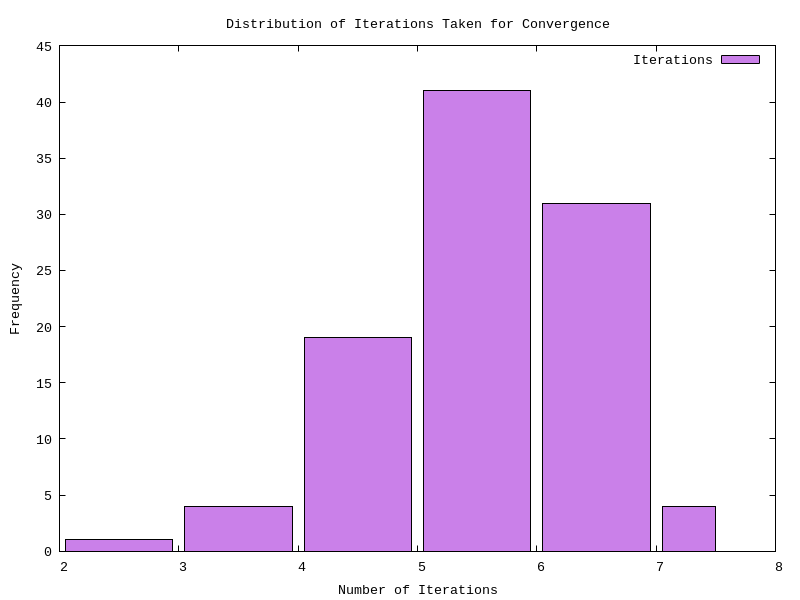
\includegraphics[width=0.75\linewidth]{../Gambar/plot_iterations_distribution.png}
    \caption{Plot Iteration taken for Convergence}
    \label{fig:iterations-distribution}
\end{figure}

\begin{figure}[H]
    \centering
    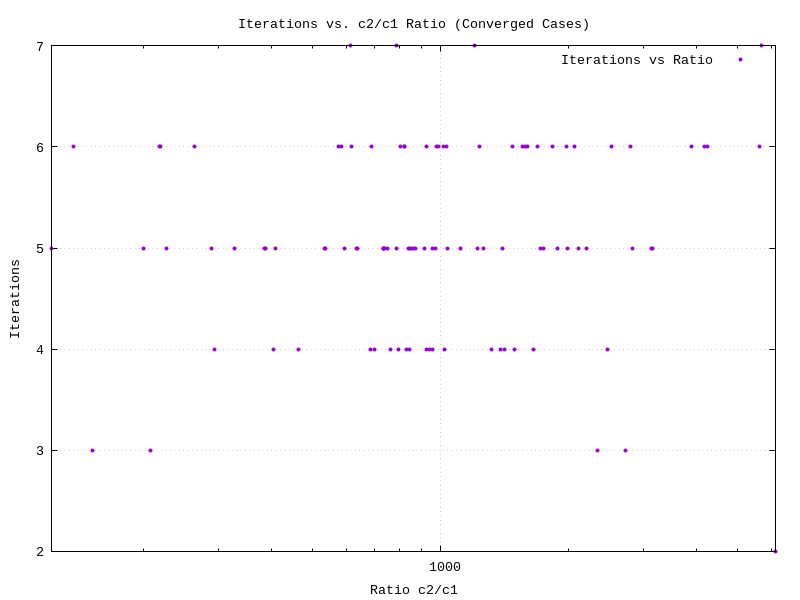
\includegraphics[width=0.75\linewidth]{../Gambar/plot_iterations_vs_c2_c1_ratio.png}
    \caption{Iteration VS c2/c1 Ratio Converged Cases}
    \label{fig:iterations-vs-ratio}
\end{figure}

\begin{figure}[H]
    \centering
    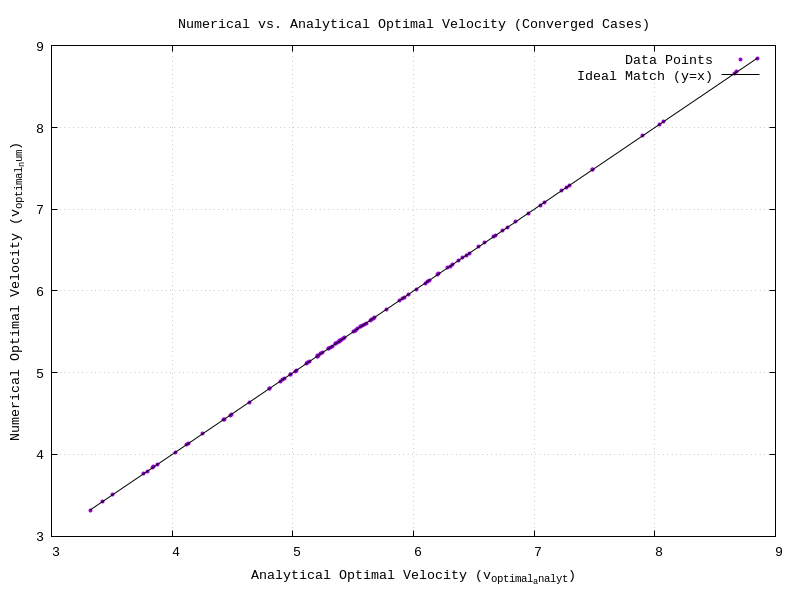
\includegraphics[width=0.75\linewidth]{../Gambar/plot_numerical_vs_analytical_velocity.png}
    \caption{Numerical VS Analytical Optimal Velocity}
    \label{fig:numerical-vs-analytical}
\end{figure}

\begin{figure}[H]
    \centering
    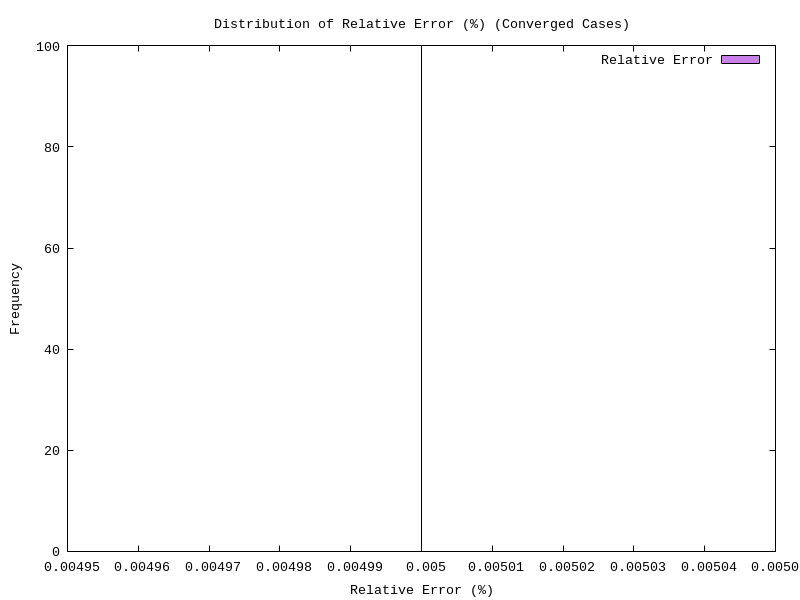
\includegraphics[width=0.75\linewidth]{../Gambar/plot_relative_error_distribution.png}
    \caption{Distribution of Relative Error}
    \label{fig:relative-error-distribution}
\end{figure}

\begin{figure}[H]
    \centering
    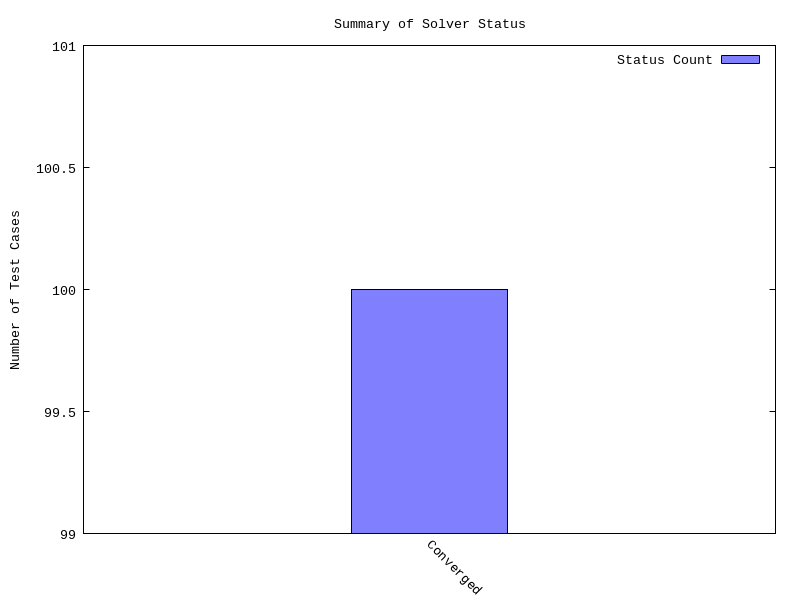
\includegraphics[width=0.75\linewidth]{../Gambar/plot_solver_status_summary.png}
    \caption{Solver Status Summary}
    \label{fig:solver-status-summary}
\end{figure}

\section{Kesimpulan}
Implementasi metode Newton-Raphson dalam C++ berhasil menentukan kecepatan optimal drone untuk memaksimalkan jangkauan dengan akurasi yang tinggi. Program membaca parameter dari file data sintetis, memungkinkan pengujian yang fleksibel. Metode ini menunjukkan konvergensi yang cepat dalam beberapa iterasi untuk berbagai set parameter, menegaskan efisiensinya untuk aplikasi optimasi parameter penerbangan drone. Penanganan berbagai kondisi batas dan error juga telah diimplementasikan untuk meningkatkan robustisitas solusi.

\section*{Link Github}
https://github.com/vinend/PemrogramanB-Kelompok7

\section*{Link Youtube}
https://youtu.be/al-s5EZC1Fg

\begin{thebibliography}{00}
\bibitem{b1} Chapman, S. J. (2023). \textit{Fortran for Sciennya untuk aplikasi optimasi parameter penerbangan drone. Petists and Engineers} (5th ed.). McGraw Hill.
\bibitem{b2} Press, W. H., Teukolsky, S. A., Vetterling, W. T., \& Flannery, B. P. (2007). \textit{Numerical Recipes: The Art of Scientific Computing} (3rd ed.). Cambridge University Press.
% Tambahkan referensi lain jika ada
\end{thebibliography}

\end{document}
